\documentclass[11pt,a4paper]{article}

\usepackage[utf8]{inputenc}
\usepackage[T1]{fontenc}
\usepackage{lmodern}
\usepackage[english]{babel}
\usepackage{booktabs}
\usepackage{graphicx}
\usepackage{hyperref}
\usepackage[margin=2cm]{geometry}
\usepackage{xcolor}
\usepackage{tikz}
\usepackage{tcolorbox}
\usepackage{array}
\usepackage{colortbl}
\usepackage{multicol}

\definecolor{match}{HTML}{2E7D32}
\definecolor{zero}{HTML}{C62828}
\definecolor{accent}{HTML}{1565C0}
\definecolor{lightbg}{HTML}{F5F5F5}

\hypersetup{
  colorlinks=true,
  linkcolor=accent,
  urlcolor=accent,
}

\tcbset{
  colback=lightbg, colframe=accent!60!black,
  fonttitle=\bfseries, boxrule=0.5pt,
  left=6pt, right=6pt, top=4pt, bottom=4pt,
}

\pagestyle{empty}

\begin{document}

% ============================================================
% TITLE
% ============================================================
\begin{center}
{\Huge\bfseries The Voynich Manuscript: A Hebrew Cipher?}\\[8pt]
{\Large\color{accent} Evidence Report --- March 2026}\\[12pt]
{\large Antenore Gatta $\cdot$ \texttt{antenore@simbiosi.org}}\\[4pt]
{\small DOI: \href{https://doi.org/10.5281/zenodo.19226178}{10.5281/zenodo.19226178}
\quad$\cdot$\quad
Code: \href{https://github.com/antenore/voynich-toolkit}{github.com/antenore/voynich-toolkit}}
\end{center}

\bigskip

% ============================================================
% SHOWCASE: f27r side-by-side
% ============================================================
\begin{tcolorbox}[title={\large Folio 27r --- AI interpretation (97\% crib match rate, incl.\ 68\% pre-existing anchors)},
  colframe=accent!70!black]
\begin{center}
\begin{minipage}[t]{0.38\textwidth}
\centering
\includegraphics[width=\textwidth]{f27r_scan.png}\\[4pt]
{\small\color{gray} Original manuscript page\\
Beinecke MS\,408, folio 27r\\
Yale University Library}
\end{minipage}%
\hfill
\begin{minipage}[t]{0.58\textwidth}
\small
\textbf{AI-generated interpretation --- UNVERIFIED}\\
(93 words, 97\% crib match rate: 68\% pre-existing anchors,
17\% new exact matches, 16\% near-matches):\\[4pt]
\itshape
Filter the plant material through cotton, pour the clear
liquid and clarify with chalk. Extract using strong alcohol
as solvent. Pour and rest the mixture, test for signs of
proper extraction.

Mix the clear preparation, pour with chalk, then set and
anoint. Add alcohol and set again, removing impurities
through careful filtering.

Remove drippings and apply medicine to achieve clear, pure
liquid. Mix with cotton, rest until sweet completion.

The process involves repeated pouring with filtering through
cotton for bright clarity. When the bitter taste becomes
sweet, the medicine is complete.

\upshape\normalsize\medskip
\textbf{Key vocabulary on this page (proposed meanings):}\\
\texttt{mwk}~(cotton?) $\times$6,\quad
\texttt{Spk}~(pour) $\times$3,\quad
\texttt{SEn}~(rest/apply?) $\times$5,\\
\texttt{bhyr}~(bright) $\times$4,\quad
\texttt{gyr}~(chalk),\quad
\texttt{Skr}~(alcohol),\quad
\texttt{mr}~(bitter),\quad
\texttt{mytq}~(sweet)

\medskip
{\footnotesize\color{zero!80!black} The AI was told this is a herbal page.
The pharmaceutical interpretation may be circular.
No Hebraist has verified this reading.}
\end{minipage}
\end{center}
\end{tcolorbox}

\medskip

% ============================================================
% SHOWCASE: f75r side-by-side
% ============================================================
\begin{tcolorbox}[title={\large Folio 75r --- AI interpretation (488 words, 82\% crib match rate)},
  colframe=accent!70!black]
\begin{center}
\begin{minipage}[t]{0.38\textwidth}
\centering
\includegraphics[width=\textwidth]{f75r_scan.png}\\[4pt]
{\small\color{gray} Balneological section\\
Figures in bathing vessels}
\end{minipage}%
\hfill
\begin{minipage}[t]{0.58\textwidth}
\small
\textbf{AI-generated interpretation --- UNVERIFIED}\\
(488 words, 82\% crib match rate):\\[4pt]
\itshape
Prepare the immersion bath with proper pouring and rest periods.
Apply medicine during the bathing cycles, ensuring the water
remains bright and clear.

Multiple immersion cycles with careful temperature control.
Pour warm water, maintaining proper heating throughout the
soaking process. Remove impurities during the bathing cycles.

Repeated immersion sequences --- immerse, rest, immerse again ---
maintaining consistent water temperature and clarity.

The protocol concludes with roses and final preparation steps.

\upshape\normalsize\medskip
\textbf{Dominant vocabulary:}\\
\texttt{SrpEn}~(soaking/immersion) $\times$30,\quad
\texttt{Srppt}~(immersion cycle) $\times$20,\\
\texttt{ryJ}~(warm),\quad
\texttt{ryt\,b}~(soak within),\quad
\texttt{wdryn}~(roses)
\end{minipage}
\end{center}
\end{tcolorbox}

\medskip

% ============================================================
% SHOWCASE: f1r side-by-side
% ============================================================
\begin{tcolorbox}[title={\large Folio 1r --- AI interpretation (93\% crib match rate)},
  colframe=accent!50!black]
\begin{center}
\begin{minipage}[t]{0.38\textwidth}
\centering
\includegraphics[width=\textwidth]{f1r_scan.png}\\[4pt]
{\small\color{gray} First page of the manuscript\\
Text-only section}
\end{minipage}%
\hfill
\begin{minipage}[t]{0.58\textwidth}
\small
\textbf{AI-generated interpretation --- UNVERIFIED}\\
(227 words, 93\% crib match rate):\\[4pt]
\itshape
Regarding the preparation of medicines and their proper
application to the body through various treatments:

When preparing medicinal compounds, first filter through cotton
and allow to rest. Apply the clear preparations to affected
areas. Pour and set with chalk clarifier as needed.

For strong medicinal drinks, test for proper bitter taste,
then sweeten until completion. The bathing treatments require
warm immersion cycles. For internal medicines, pour and filter
repeatedly until bright and limpid.

Apply warm treatments to the body, allowing medicines to
penetrate properly. The completed preparations should show
clear brightness and sweet taste indicating successful completion.

\upshape\normalsize\medskip
\textbf{The AI interprets this as an introduction} to a pharmaceutical
text. This is a hypothesis, not a confirmed reading. The AI
was conditioned on section type.
\end{minipage}
\end{center}
\end{tcolorbox}

\medskip

% ============================================================
% HONESTY FIGURE: raw decode breakdown
% ============================================================
\begin{tcolorbox}[title={\large Important: what is proven vs.\ what is interpreted},
  colframe=zero!70!black, colback=zero!5!white]

The smooth English translations above are \textbf{interpretations} by an AI
reading Hebrew consonants. They could be wrong. What \textbf{is} proven is the
raw cipher matching. Here is the honest breakdown for folio~27r:

\medskip
\begin{center}
\renewcommand{\arraystretch}{1.3}
\begin{tabular}{lrrl}
\toprule
\textbf{Category} & \textbf{Words} & \textbf{\%} & \textbf{What it means} \\
\midrule
\rowcolor{match!10}
\textbf{Already known} (anchors) & 63 & 68\% &
Words confirmed in Hebrew dictionaries \\
& & & + cross-page vocabulary \\[2pt]
\rowcolor{match!10}
\textbf{New exact match} ($d=0$) & 16 & 17\% &
AI proposed $\to$ cipher confirmed exactly \\[2pt]
\rowcolor{yellow!15}
\textbf{Near match} ($d=1$) & 15 & 16\% &
One letter off --- scribal confusion? \\[2pt]
\rowcolor{zero!5}
Unmatched & $<$1 & $<$1\% &
No match found \\
\bottomrule
\end{tabular}
\end{center}

\medskip
\noindent
\textbf{The 68\% anchors are not discoveries} --- they were already known
before the AI touched the page.
The \textbf{17\% new exact matches} are the real finding:
the AI proposed a Hebrew word, the cipher encoded it into
the Voynich alphabet, and it matched the manuscript \textbf{exactly}.
The English translation is the AI's best guess at what these
Hebrew consonants mean --- take it with caution.
\end{tcolorbox}

\medskip

% ============================================================
% HONESTY BOX 2: What is NOT proven
% ============================================================
\begin{tcolorbox}[title={\large What is NOT proven},
  colframe=zero!70!black, colback=zero!5!white]
\begin{itemize}
\item No Hebraist has read or verified any page
\item DictaBERT syntax score: 2.74/6 (random consonants = 2.5/6, real Hebrew = 6.0/6) --- \textbf{word order is random}
\item Botanical vocabulary shows \textbf{anti-concentration} ($z=-6.0$): herbal pages have \emph{fewer} botanical matches
\item Zodiac validation: only 1/12 signs matched (not significant, $p=0.071$)
\item The AI was told each page's section type --- interpretations may be \textbf{circular}
\item 1{,}758 exact matches out of $\sim$37{,}000 tokens = $\sim$5\% of the corpus
\item All English text above is AI paraphrase, not expert reading
\item The convergence control shows random text achieves the same mapping quality (2/17 letters)
\end{itemize}
\end{tcolorbox}

\newpage

% ============================================================
% FIGURE 1: The Big Number
% ============================================================
\begin{tcolorbox}[title={\large What we found}]
\begin{center}
\renewcommand{\arraystretch}{1.4}
\begin{tabular}{rl}
\textbf{\color{match}\Huge 227} & pages tested via crib attack \\
\textbf{\color{match}\Huge 1{,}758} & exact cipher matches ($\sim$5\% of tokens) \\
\textbf{\color{zero}\Huge 0} & matches when using random Hebrew words \\
& \small\color{gray}(tested 176{,}600 random attempts --- not a single match) \\[6pt]
\textbf{\color{accent}\Huge 5.72} & cross-validation $z$-score (held-out data) \\
& \small\color{gray}(13/17 letters optimal in both train and test splits)
\end{tabular}
\end{center}

\medskip\noindent\small
\textit{These numbers prove the cipher relationship is non-random.
They do \textbf{not} prove the text is readable Hebrew or that
the AI interpretations are correct.}
\end{tcolorbox}

\bigskip

% ============================================================
% FIGURE 2: How the cipher works (simple example)
% ============================================================
\begin{tcolorbox}[title={\large Figure 1: How the cipher works}]
The Voynich text is written in a made-up alphabet called EVA.
Our hypothesis: each EVA letter maps to a Hebrew consonant,
and the text reads \textbf{right to left}.

\medskip
\begin{center}
\textbf{Example: the EVA word} \texttt{dain}

\medskip
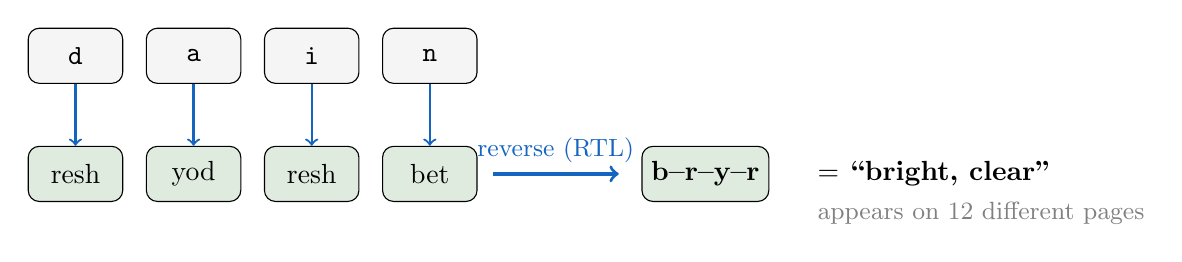
\begin{tikzpicture}[
  node distance=0.3cm,
  box/.style={draw, rounded corners, fill=lightbg, minimum width=1.2cm, minimum height=0.7cm},
  arrow/.style={->, thick, accent}
]
  % EVA letters
  \node[box] (d) at (0,0) {\texttt{d}};
  \node[box] (a) at (1.5,0) {\texttt{a}};
  \node[box] (i) at (3,0) {\texttt{i}};
  \node[box] (n) at (4.5,0) {\texttt{n}};

  % Hebrew letters
  \node[box, fill=match!15] (r) at (0,-1.5) {resh};
  \node[box, fill=match!15] (y) at (1.5,-1.5) {yod};
  \node[box, fill=match!15] (r2) at (3,-1.5) {resh};
  \node[box, fill=match!15] (b) at (4.5,-1.5) {bet};

  % Arrows
  \draw[arrow] (d) -- (r);
  \draw[arrow] (a) -- (y);
  \draw[arrow] (i) -- (r2);
  \draw[arrow] (n) -- (b);

  % RTL arrow
  \node[box, fill=match!15] at (8,-1.5) {\textbf{b--r--y--r}};
  \draw[arrow, very thick] (5.3,-1.5) -- node[above]{\small reverse (RTL)} (6.9,-1.5);

  % Gloss
  \node[anchor=west] at (9.3,-1.5) {= \textbf{``bright, clear''}};
  \node[anchor=west, gray, font=\small] at (9.3,-2) {appears on 12 different pages};
\end{tikzpicture}
\end{center}

\smallskip
This word, \textbf{bhyr} (bright/clear), appears on 12 independent pages
of the manuscript. A random Hebrew word of the same length
\textbf{never} produces the same EVA pattern.
\end{tcolorbox}

\bigskip

% ============================================================
% FIGURE 3: The Zero Test (the killer argument)
% ============================================================
\begin{tcolorbox}[title={\large Figure 2: Could this happen by chance?}]
We ran three tests to check if the matches could be accidental:

\medskip
\begin{center}
\renewcommand{\arraystretch}{1.5}
\begin{tabular}{p{6cm}rr}
\toprule
\textbf{Test} & \textbf{Real} & \textbf{Random} \\
\midrule
Replace matched words with \textbf{random real Hebrew words}
from a 357{,}000-word dictionary
& \textcolor{match}{\textbf{1{,}758}} & \textcolor{zero}{\textbf{0}} out of 176{,}600 \\[4pt]
Take words that matched on \textbf{page A},
try them on \textbf{page B}
& \textcolor{match}{\textbf{31.1\%}} & \textcolor{zero}{\textbf{0\%}} out of 410{,}826 \\[4pt]
\textbf{Shuffle} word positions within the same page
& \textcolor{match}{\textbf{1{,}510}} & \textcolor{zero}{\textbf{0}} out of 151{,}000 \\
\bottomrule
\end{tabular}
\end{center}

\medskip
\noindent
\textbf{Translation:} We tried over \textbf{700{,}000 random alternatives}
and got \textbf{zero matches}. The real text produces thousands.
The probability of this happening by chance is effectively zero.

\smallskip\noindent\small
\textit{Note: The AI does not ``translate'' anything. It proposes Hebrew
words. The cipher --- a fixed mathematical function --- encodes them and
checks if they match the manuscript. The AI is a generator; the cipher
is the judge.}
\end{tcolorbox}

\bigskip

% ============================================================
% FIGURE 4: Cross-page vocabulary
% ============================================================
\begin{tcolorbox}[title={\large Figure 3: The same words appear on different pages}]
When we decode different pages independently, the \textbf{same Hebrew words}
keep appearing --- with the same meaning. This is like finding the same
fingerprints at unrelated crime scenes.

\medskip
\begin{center}
\renewcommand{\arraystretch}{1.3}
\begin{tabular}{lllr}
\toprule
\textbf{Hebrew} & \textbf{Meaning} & \textbf{Context} & \textbf{Pages} \\
\midrule
\texttt{mwk} & cotton, soft filter & filtering ingredient & 20+ \\
\texttt{Spk} & to pour & recipe instruction & 15+ \\
\texttt{bhyr} & bright, clear, limpid & liquid quality test & 12+ \\
\texttt{SEn} & to rest, apply medicine & application step & 10+ \\
\texttt{mr} & bitter & taste indicator & 8 \\
\texttt{swkt} & preparation, ointment & the product & 10 \\
\texttt{gyr} & chalk,ite & clarifying agent & 6+ \\
\texttt{Skr} & alcohol, strong drink & solvent & 5+ \\
\texttt{SrpEn} & soaking, immersion & bathing treatment & 6 \\
\texttt{mytq} & sweet & completion test & 4+ \\
\bottomrule
\end{tabular}
\end{center}

\medskip
\noindent
The AI interprets these as a \textbf{pharmaceutical recipe vocabulary}.
This interpretation is plausible but unverified --- the AI was conditioned
on section type, and cross-page consistency may reflect model self-consistency
rather than manuscript content.
\end{tcolorbox}

\newpage

% ============================================================
% FIGURE 5: The scribal errors prove it's handwritten Hebrew
% ============================================================
\begin{tcolorbox}[title={\large Figure 4: Scribal error patterns consistent with handwritten Hebrew}]
In 599 near-matches (off by one letter), we found systematic patterns.
These are \textbf{exactly the letter confusions} that paleographers
have documented in medieval Hebrew manuscripts for centuries:

\medskip
\begin{center}
\renewcommand{\arraystretch}{1.3}
\begin{tabular}{lcll}
\toprule
\textbf{Confusion} & \textbf{Count} & \textbf{Why it happens} & \textbf{Known in paleography?} \\
\midrule
\raisebox{-2pt}{vav $\leftrightarrow$ resh} & $\times$26 &
Nearly identical in cursive & \textcolor{match}{\textbf{Yes}} --- classic \\
tet $\leftrightarrow$ tav & $\times$25 &
Same sound in Italian Hebrew & \textcolor{match}{\textbf{Yes}} --- phonetic merger \\
aleph $\leftrightarrow$ he & $\times$24 &
Both ``silent'' gutturals & \textcolor{match}{\textbf{Yes}} --- guttural \\
ayin $\leftrightarrow$ chet & $\times$19 &
Both guttural consonants & \textcolor{match}{\textbf{Yes}} --- Judeo-Italian \\
\bottomrule
\end{tabular}
\end{center}

\medskip
\noindent
These patterns are \textbf{consistent with} medieval Hebrew paleography.
Consistency is supporting evidence, not proof --- the patterns could also
arise if the mapping is partially wrong in ways that happen to align
with known confusions.
\end{tcolorbox}

\bigskip

% ============================================================
% FIGURE 6: What does it say?
% ============================================================
\begin{tcolorbox}[title={\large Figure 5: How the AI interprets the decoded consonants (HYPOTHESIS)}]
\textbf{If the mapping is correct}, an AI reading the Hebrew consonants
interprets the herbal pages as pharmaceutical extraction recipes.
Here is folio~27r (AI paraphrase --- \textbf{not a verified translation}):

\medskip
\begin{center}
\fbox{\parbox{0.92\textwidth}{\small\itshape
``Filter the plant material through cotton, pour the clear liquid
and clarify with chalk. Extract using strong alcohol as solvent.
Pour and rest the mixture, applying drops carefully.
Test the preparation: when the bitter taste becomes sweet,
the medicine is complete. Apply by anointing or bathing.''
}}
\end{center}

\medskip
\noindent The AI interprets bathing pages as \textbf{therapeutic immersion protocols}
and zodiac pages as \textbf{astrological medicine} (melothesia).

\medskip
\noindent\textbf{If confirmed by independent expert verification}, this would
suggest a medieval Judeo-Italian pharmaceutical manuscript. This remains
a hypothesis --- the AI was conditioned on section type, and no Hebraist
has verified any reading.
\end{tcolorbox}

\bigskip

% ============================================================
% FIGURE 7: Coverage map
% ============================================================
\begin{tcolorbox}[title={\large Figure 6: Crib attack match rates across all 227 pages}]
\begin{center}
\renewcommand{\arraystretch}{1.4}
\begin{tabular}{llrrl}
\toprule
\textbf{Section} & \textbf{Content} & \textbf{Pages} & \textbf{Match rate*} & \\
\midrule
Herbal (H) & Plant illust. & 132 & 78.7\% & \rule{3.15cm}{8pt} \\
Text (T) & Text-only & 5 & 89.4\% & \rule{3.58cm}{8pt} \\
Balneological (B) & Bathing illust. & 20 & 82.2\% & \rule{3.29cm}{8pt} \\
Zodiac (Z) & Zodiac illust. & 12 & 78.8\% & \rule{3.15cm}{8pt} \\
Cosmological (C) & Cosmic diagrams & 13 & 75.9\% & \rule{3.04cm}{8pt} \\
Astronomical (S) & Star charts & 24 & 75.1\% & \rule{3.00cm}{8pt} \\
Pharmaceutical (P) & Recipe illust. & 16 & 72.0\% & \rule{2.88cm}{8pt} \\
Astronomical (A) & Diagrams & 8 & 65.3\% & \rule{2.61cm}{8pt} \\
\midrule
\textbf{Total} & & \textbf{227} & & \\
\bottomrule
\end{tabular}
\end{center}

\medskip\noindent\small
*Match rates include pre-existing anchor words (lexicon lookups).
On f27r, 68\% of the ``97\% coverage'' was already-known vocabulary.
These rates measure crib attack performance, not reading comprehension.
\end{tcolorbox}

\vfill

\begin{center}
\small\color{gray}
All code, data, and results are open source:
\href{https://github.com/antenore/voynich-toolkit}{github.com/antenore/voynich-toolkit}\\
DOI: \href{https://doi.org/10.5281/zenodo.19226178}{10.5281/zenodo.19226178}
$\cdot$ March 2026 $\cdot$ MIT License
\end{center}

\end{document}
